\documentclass{beamer}
\usetheme{Boadilla}

\usepackage{tikz}
\usepackage{siunitx}
\usepackage{graphicx}

\graphicspath{{img/}}

\title[Physics Problem Solving]{Physics Problem Solving}
\author[Dara \and Eason \and Lev]{Dara Daneshvar \and Eason Shao \and Lev Shabalin}
\institute[St Paul's School]{Physics Problem Solving Society\\St Paul's School}
\date{16.09.2024}

\AtBeginSection[]
{
    \frame{
        \frametitle{Table of Contents}
        \tableofcontents[currentsection]
    }
}

\begin{document}

\frame{\titlepage}

\frame{
    \frametitle{Table of Contents}
    \tableofcontents
}

\section{Waves and Energy}

\frame{
    \frametitle{Reflection of Waves}

    The diagram shows the effect of touching the centre of the surface of water in a glass.

    \begin{columns}
        \begin{column}{0.7\textwidth}
            \begin{block}{Qu (3) a, b: [2 + 1]}
                \begin{enumerate}
                    \item Draw a series of four sketches to show the motion of a single circular ripple, viewed from above, from the time it is generated at the centre to the time it returns to the centre. Include arrows to show the direction of the ripple.
                    \item Explain why the amplitude of the ripple reduces as the ripple travels outwards and its radius increases.
                \end{enumerate}
            \end{block}
        \end{column}

        \begin{column}{0.3\textwidth}
            \begin{figure}
                \centering
                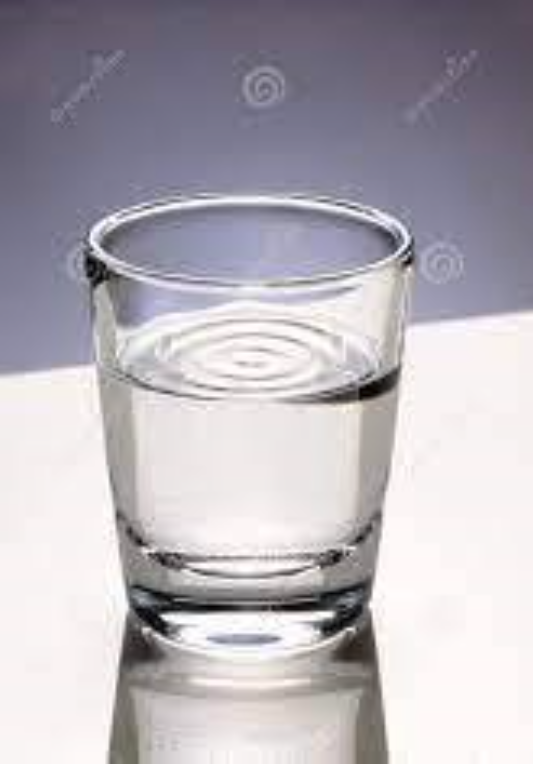
\includegraphics[scale=0.1]{glass_water.png}
                \caption{Surface of water in a glass disturbed by touching by a finger.}
            \end{figure}
        \end{column}

    \end{columns}
}

\frame{
    \begin{definition}[Intensity of a Wave]
        The intensity of a progressive wave, \(I\), is defined by the amount of energy passing through a unit area per unit time:\pause
        \[
            I = \frac{P}{S}
        \]\pause
        where \(I\) is intensity with SI unit \(\si{\watt\per\metre\squared}\), \(P\) is the power with SI unit \(\si{\watt}\) and \(S\) is the area with SI unit \(\si{\metre\squared}\).
    \end{definition}\pause

    \begin{fact}[Relations on Intensities]
        We have that the intensity of a progressive wave is proportinal to its amplitude \(A\) squared:
        \[
            I \propto A^2,
        \]\pause
        and that it is also proportional to its frequency squared:
        \[
            I \propto f^2.
        \]
    \end{fact}
}

\frame{
    \begin{fact}[Relations on Intensities]
        We have that the intensity of a progressive wave is proportinal to its amplitude \(A\) squared:
        \[
            I \propto A^2.
        \]
    \end{fact}

    \begin{proof}\pause
        Energy transferred in a wave is due to work done to create the wave. \pause

        The larger the displacement \(x\), the larger the force \(F = kx\) is used to create it. (We assume simple linearlity situation now, such as in Hooke's Law.)\pause

        The work done \(W\) is equal to the force \(F\) multiplied by the distance \(x\), and therefore
        \[
            F = kx^2,
        \]
        and the proportionality to the amplitude squared is now demonstrated.
    \end{proof}
}

\section{Lenses}

\frame{
    \frametitle{Convex Lens and Curvature}

    This situation is analogous to the focussing effect of a circular mirror. Here the object is the initial contact with the water and the (real) image is at the final point of convergence of the ripple.

    Another, familiar situation in which image distance equals object distance is shown. (The lens is assumed to be thin for the purpose of drawing rays.)

    \begin{figure}
        \centering
        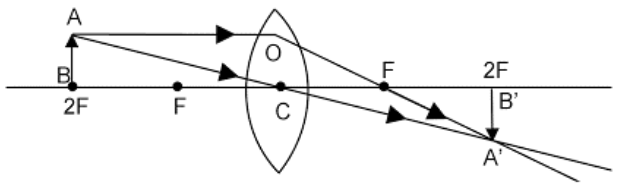
\includegraphics[scale=0.25]{converging_lens.png}
        \caption{Ray diagram for a thin converging lens.}
    \end{figure}

    \begin{block}{Qu (4) c: [2]}
        Explain how this lens behaviour resembles the reflecting behaviour of a circular mirror and use your explanation to state the relationship between the focal length of a mirror and its radius of curvature.
    \end{block}
}

\frame{
    \begin{fact}[Three/Two Special Lines]
        \begin{itemize}\pause
            \item A ray that was parallel to the optical axis will pass through one of the focal points after the lens.\pause
            \item A ray which passes through the optical centre remains unbent.\pause
            \item A ray which passed through a focal point will be parallel to the optical axis after the lens.\pause
        \end{itemize}
    \end{fact}

    Consider thin convex lens with focal distance \(f\) and object distance \(u\).\pause

    Draw diagrams for the following relations. \pause Think about whether the image is: (1) real or virtual, (2) upright or inverted, (3) enlarged or diminished:
    \begin{itemize}
        \item \(0 < u < f\),
        \item \(u = f\),
        \item \(f < u < 2f\),
        \item \(u = 2f\),
        \item \(2f < u\).
    \end{itemize}
}

\frame{
    \begin{fact}[Gaussian Mirror Equation]
        For thin lenses with object distance \(u\), image distance \(v\) and focal distance \(f\):\pause
        \[
            \frac{1}{u} + \frac{1}{v} = \frac{1}{f}.
        \]\pause

        Note that, by convention, concave lens have \(f < 0\) and convex lens have \(f > 0\); real images have \(v > 0\) and virtual images have \(v < 0\).\pause

        This also holds for convex and concave mirrors!\pause
    \end{fact}

    \begin{definition}[Linear Magnification]
        The linear magnification \(M\) of an imaging system is given by
        \[
            M = - \frac{v}{u}.
        \]\pause

        \(M > 0\) for upright images, and \(M < 0\) for inverted images.
    \end{definition}
}

\section{Geometry}

\frame{
    \frametitle{Parabola and Light}

    A better focussing geometry is given by a parabolic mirror.

    The standard equation of a parabola is
    \[
        y^2 = 4ax
    \]
    where \(a\) is the so-called focal distance of the parabola.

    \begin{block}{Qu (4) d, e: [2 + 6]}
        \begin{enumerate}
            \item Sketch a graph of the function \(y^2 = 4ax\). This must occupy at least half a page.
                  Add to your sketch a light ray parallel to the \(x\)--axis, meeting the parabola at the general
                  point \((X, Y)\).
            \item Show mathematically that this arbitrary ray is reflected through the point \((a, 0)\) and so
                  justify describing \(a\) as the focal distance.
        \end{enumerate}
    \end{block}
}

\frame{
    \begin{fact}[Optical Properties of Conic Sections/Quadratic Curves]
        \begin{itemize}\pause
            \item Rays emitted from one of the foci of an ellipse will end up in the other focus, after exactly one reflection on the ellipse. \href{https://www.desmos.com/calculator/tp9cmmsiwl}{\beamergotobutton{Ellipse}}\pause
            \item Rays emitted from the focus of a parabola will end up parallel to the axis, after exactly one reflection on the parabola. \href{https://www.desmos.com/calculator/9e4ve2oltk}{\beamergotobutton{Parabola}}\pause
            \item Rays emitted from one of the foci of a hyperbola will end up emmiting from the other focus, after exactly one reflection on either branch of the hyperbola. \href{https://www.desmos.com/calculator/bigabvtswp}{\beamergotobutton{+ve Branch}} \href{https://www.desmos.com/calculator/hb85fp0vep}{\beamergotobutton{-ve Branch}}
        \end{itemize}
    \end{fact}
}

\end{document}